\documentclass[conference]{IEEEtran}
\IEEEoverridecommandlockouts
% Template-aligned conference preamble with XeLaTeX support for Chinese
\usepackage{fontspec}
\defaultfontfeatures{Ligatures=TeX}
\setmainfont{SimSun}[AutoFakeBold=2.0, AutoFakeSlant=0.2]
\setsansfont{Microsoft YaHei}[AutoFakeBold=2.0, AutoFakeSlant=0.2]
\setmonofont{Consolas}
\XeTeXlinebreaklocale "zh"
\XeTeXlinebreakskip = 0pt plus 1pt
\usepackage{cite}
\usepackage{amsmath,amssymb,amsfonts}
\interdisplaylinepenalty=2500
\usepackage{algorithmic}
\usepackage{algorithm}
\usepackage{graphicx}
\usepackage{textcomp}
\usepackage{xcolor}
\renewcommand{\abstractname}{摘要}
\renewcommand{\IEEEkeywordsname}{关键词}
\renewcommand{\figurename}{图}
\renewcommand{\tablename}{表}
\renewcommand{\refname}{参考文献}
\floatname{algorithm}{算法}
\renewcommand{\algorithmicrequire}{\textbf{输入:}}
\renewcommand{\algorithmicensure}{\textbf{输出:}}
\renewcommand{\algorithmicreturn}{\textbf{返回}}
\renewcommand{\algorithmicif}{\textbf{如果}}
\renewcommand{\algorithmicthen}{\textbf{则}}
\renewcommand{\algorithmicelse}{\textbf{否则}}
\renewcommand{\algorithmicelsif}{\algorithmicelse\ \algorithmicif}
\renewcommand{\algorithmicendif}{\textbf{结束如果}}
\renewcommand{\algorithmicfor}{\textbf{对于}}
\renewcommand{\algorithmicdo}{\textbf{执行}}
\renewcommand{\algorithmicendfor}{\textbf{结束循环}}
\def\BibTeX{{\rm B\kern-.05em{\sc i\kern-.025em b}\kern-.08em
    T\kern-.1667em\lower.7ex\hbox{E}\kern-.125emX}}
\begin{document}
\title{基于实时预约数据库的智能停车分配与减少寻位巡游系统}

\author{
    \IEEEauthorblockN{1\textsuperscript{st} Haonan Cheng}
    \IEEEauthorblockA{\textit{计算机科学与技术系} \\
        \textit{亚洲大学 ICT 研究生院}\\
        韩国水原 \\
        haonan.cheng@hotmail.com}
    \and
    \IEEEauthorblockN{2\textsuperscript{nd} Mingyuan Zhou}
    \IEEEauthorblockA{\textit{计算机科学与技术系} \\
        \textit{亚洲大学 ICT 研究生院}\\
        韩国水原 \\
        ruyezhou020726@gmail.com}
}

\maketitle

\begin{abstract}
城市交通拥堵会因车辆为寻找停车位而持续巡游而显著加剧，这一过程会额外消耗燃油、增加排放并降低路网运行效率。本文提出一个基于 SUMO、Python TraCI 与 PostgreSQL 的智能停车分配与减少寻位巡游系统。控制器以 Python 字典维护预约状态，将停车库存与场景汇总同步到关系型数据表，并在局部占用率超过 70\% 与 90\% 时执行分层动态定价。基于数据库结果，场景 A 在 7,200~s 仿真上限时停放了 2,500 辆计划车辆中的 2,498 辆，而场景 B 在 3,922~s 完成全部 2,500 辆车停放，同时降低了平均寻位时间、燃油消耗和部分排放指标。
\end{abstract}

\begin{IEEEkeywords}
    智能停车，停车寻位巡游，微观交通仿真，SUMO，关系型数据库，动态定价，Python TraCI，PostgreSQL。
\end{IEEEkeywords}

\section{引言}
随着全球城市化进程加速，城市出行正面临前所未有的挑战。交通拥堵的一个普遍诱因是“为寻找停车位而巡游” \cite{b1}。在中央商务区（CBD）中，高峰时段的巡游车辆可占总交通量的 20\% 到 30\% \cite{b2}。

传统停车管理依赖静态标志或局部 IoT 传感器网络 \cite{b3}。这些方法虽然可以提供实时状态，但缺乏系统级的主动协同能力。当多辆车同时瞄准同一个可用车位时，局部瓶颈随之出现，未能成功停车的驾驶员被迫重新巡游。

为解决这一问题，现代智能交通系统（ITS）必须从“被动搜索”转向“主动预约” \cite{b4}。然而，在微观层面仿真并实现此类系统会带来巨大的计算挑战。本文弥合了微观交通仿真与企业级数据库之间的差距。我们的核心贡献包括：

\begin{enumerate}
    \item \textbf{数学建模}: 将停车分配建模为一个在距离、费用与网络负载之间权衡的多目标优化问题。
    \item \textbf{高性能预约状态}: 在 TraCI 控制循环中使用 Python 字典处理高频预约查询，并将更新批量写入 PostgreSQL，以在不牺牲仿真速度的前提下保证持久化日志完整性。
    \item \textbf{多层级动态定价}: 实现需求响应算法，在占用率达到 70\% 和 90\% 时将基础价格分别提高到 1.5 倍和 2.0 倍，从而自然地将交通引导至外围停车场。
    \item \textbf{微观评估}: 利用 TraCI 接口仿真 2,500 条计划行程，并通过执行时相同的监控流水线量化完成时间、搜索时间、燃油消耗、显式巡航距离、部分排放指标和路网速度。
\end{enumerate}

\section{相关工作}

\subsection{巡游行为的建模与影响}
Shoup \cite{b1} 和 Inci \cite{b2} 记录了停车价格过低带来的经济与环境影响。然而，宏观模型往往无法捕捉路口和停车场入口处发生的复杂智能体级交互 \cite{b5}。

\subsection{智能停车与 IoT 集成}
Lin 等人 \cite{b3} 对基于传感器的停车系统进行了综述。Geng 和 Cassandras \cite{b4} 提出了基于资源分配与预约的系统。然而，许多概念性方案依赖离散事件仿真器，而非高保真的微观交通环境。

\subsection{交通领域的动态定价}
动态定价能够有效管理网约车与收费道路中的峰值需求。Fosgerau \cite{b6} 和 Pierce \cite{b7} 分析了基于利用率的停车费优化。我们将多层级定价逻辑直接嵌入仿真循环，以观察其对车辆路径选择产生的即时微观影响。

\subsection{联合仿真中的数据同步}
Wegener 等人 \cite{b8} 讨论了 TraCI 在扩展到数千辆车时的延迟瓶颈。在本项目中，TraCI 控制循环使用 Python 字典维护活跃预约状态，并按固定仿真间隔将持久化更新写入 PostgreSQL。

\section{系统架构与方法}
该架构在 SUMO 仿真、Python TraCI 控制器与 PostgreSQL 数据库之间形成闭环系统。

\begin{figure}[htbp]
    \centering
    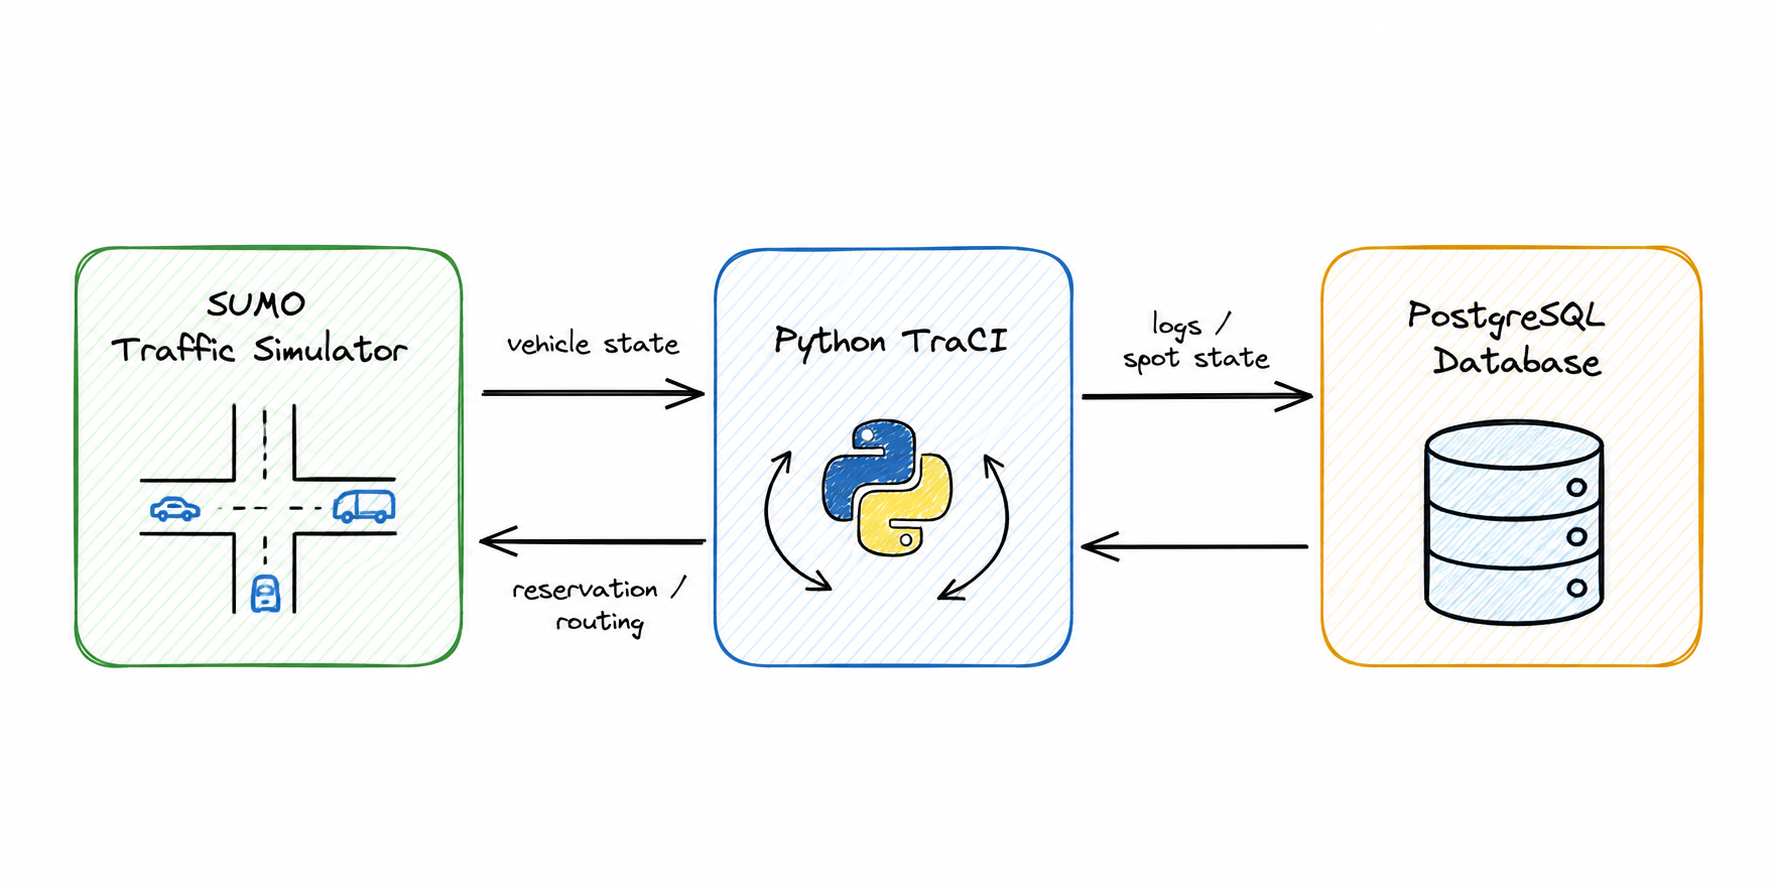
\includegraphics[width=\linewidth]{paper_assets/fig1_architecture_gpt.png}
    \caption{系统架构，展示 SUMO、Python TraCI 与 PostgreSQL 之间的数据流。}
    \label{fig:architecture}
\end{figure}

\subsection{问题建模}
目标是为车辆 $v_i \in V$ 分配最优停车位 $p_j \in P$，以最小化广义停车成本。分配逻辑如下：

\begin{enumerate}
    \item \textbf{候选车位过滤（容量约束）}:
          系统遍历预约状态字典，只有当某车位的已预约容量严格小于其总容量时，才将其加入候选列表：
          \begin{equation}
              \sum_{i \in V} x_{ij} < Capacity(p_j), \quad \forall p_j \in P
          \end{equation}

    \item \textbf{动态价格计算}:
          对每个可用车位，系统读取实时占用率 $\rho$。当前价格 $Price(p_j)$ 会根据 70\% 和 90\% 的占用率阈值进行调整。

    \item \textbf{成本评估（成本函数）}:
          候选车位 $p_j$ 的广义停车成本 $C_{ij}$ 统一表示为货币成本：
          \begin{equation}
              C_{ij} = Price(p_j) + d_{route}(v_i, p_j) \cdot c_d
          \end{equation}
          其中，$d_{route}$ 表示车辆到停车区的估算路网行驶距离，$c_d$ 表示每米距离折算的货币成本。实现中设置 $c_d=0.0025$，即额外行驶 1 km 约等价于 2.5 个货币单位。

    \item \textbf{贪心分配}:
          系统选取使 $C_{ij}$ 最小的候选车位，将代价较高的全局优化问题转化为面向单车的高效低延迟局部分配。
\end{enumerate}

\subsection{数据库与状态字典机制}
系统使用精简的 PostgreSQL 架构以降低事务开销，同时保留可复现实验对比所需字段：

\begin{itemize}
    \item \textbf{\texttt{parking\_spots}}: 管理停车库存以及控制逻辑使用的动态预约状态。
          \begin{itemize}
              \item \textit{静态}: \texttt{spot\_id}, \texttt{edge\_id}, \texttt{spot\_type}, \texttt{capacity} 和 \texttt{base\_price}。
              \item \textit{动态}: \texttt{occupied} 和 \texttt{current\_price}，二者由 Python 状态字典同步到数据库。
          \end{itemize}
    \item \textbf{\texttt{cruising\_logs}}: 跟踪车辆级停车行为、行驶代价和环境输出。
          \begin{itemize}
              \item \textit{核心}: \texttt{log\_id}, \texttt{vehicle\_id}, \texttt{scenario} 和 \texttt{final\_spot\_id}。
              \item \textit{运行}: \texttt{search\_time\_sec}, \texttt{cruising\_distance\_m} 和 \texttt{total\_fuel\_mg}。
              \item \textit{环境}: \texttt{total\_co2\_mg}, \texttt{total\_nox\_mg} 和 \texttt{total\_pmx\_mg}。
          \end{itemize}
    \item \textbf{\texttt{simulation\_runs}}: 保存运行级结果，包括 \texttt{completion\_time\_sec}, \texttt{total\_vehicles}, \texttt{parked\_vehicles}, \texttt{failed\_vehicles} 和 \texttt{parking\_rate}。
\end{itemize}

\textbf{基于字典的预约工作流:}
\begin{enumerate}
    \item \textbf{初始化}: 仿真开始前，将 \texttt{parking\_spots} 表加载到 Python 字典中。
    \item \textbf{仿真循环}: 预约引擎在字典中执行 $O(1)$ 查找，在内存中即时更新占用率并计算价格。
    \item \textbf{批量同步}: 每隔 60 个仿真秒，Python TraCI 控制逻辑通过 \texttt{sync\_spots} 或 \texttt{sync\_spots\_priced} 向 PostgreSQL 写入一次批量 \texttt{UPDATE} 事务。
\end{enumerate}

\begin{algorithm}[htbp]
    \caption{动态定价与预约引擎}
    \label{alg:reservation}
    \begin{algorithmic}[1]
        \REQUIRE 车辆 $v_i$，状态字典 $\mathcal{D}$
        \ENSURE 最优停车位 $p_{opt}$
        \STATE $min\_cost \gets \infty$
        \STATE $p_{opt} \gets \text{NULL}$
        \FOR{\textbf{每个} 车位 $p_j \in \mathcal{D}$}
        \IF{$p_j.\text{booked} < p_j.\text{capacity}$}
        \STATE $\rho \gets p_j.\text{booked} / p_j.\text{capacity}$
        \IF{$\rho > 0.90$}
        \STATE $P_{current} \gets p_j.\text{base\_price} \times 2.0$
        \ELSIF{$\rho > 0.70$}
        \STATE $P_{current} \gets p_j.\text{base\_price} \times 1.5$
        \ELSE
        \STATE $P_{current} \gets p_j.\text{base\_price}$
        \ENDIF
        \STATE $dist \gets \text{LocalGraphRouteDistance}(v_i, p_j)$
        \STATE $cost \gets P_{current} + (dist \times UNIT\_DIST\_COST)$
        \IF{$cost < min\_cost$}
        \STATE $min\_cost \gets cost$
        \STATE $p_{opt} \gets p_j$
        \ENDIF
        \ENDIF
        \ENDFOR
        \IF{$p_{opt} \neq \text{NULL}$}
        \STATE $p_{opt}.\text{booked} \gets p_{opt}.\text{booked} + 1$
        \STATE 将车辆 $v_i$ 经 TraCI 路由至 $p_{opt}$
        \ENDIF
        \RETURN $p_{opt}$
    \end{algorithmic}
\end{algorithm}

\subsection{多层级动态定价逻辑}
如算法 \ref{alg:reservation} 所示，当前价格 $P_{current}$ 是一个由实时局部占用率 $\rho$ 决定的分段函数：
\begin{equation}
    P_{current} =
    \begin{cases}
        P_{base},            & \text{若 } \rho \le 0.70        \\
        1.5 \times P_{base}, & \text{若 } 0.70 < \rho \le 0.90 \\
        2.0 \times P_{base}, & \text{若 } \rho > 0.90
    \end{cases}
\end{equation}

场景 B 脚本会在每个仿真步处理新出发车辆之前重新计算该分段函数。小容量路侧车位按街道聚合，阈值由 \texttt{STREET\_SPOT\_THRESHOLD=3} 控制；大容量路外枢纽则按自身的已预约容量比例定价。车辆到车位的距离由 Python 中缓存的 SUMO 路网图估算，每辆新出发车辆只执行一次 Dijkstra 搜索；成本函数使用 \texttt{UNIT\_DIST\_COST=0.0025} 将路网距离折算到与停车价格一致的货币单位。

\subsection{巡游检测与 TraCI 集成}
在基线场景中，车辆盲目行驶并直接从路网中寻找车位。基线脚本从 \texttt{demo.net.xml} 构造对向道路和出边映射，在 180 m 可视距离内扫描停车区域，每隔三个仿真步检查路口方向，并在路径即将耗尽时重新随机选路。若车辆锁定某一目标车位后 120 秒内仍无法停入，该目标会被放弃，从而再现竞争式路侧寻位中的不稳定行为。

场景 B 移除了这种沿街扫描循环。每辆新出发车辆通过内存字典完成一次分配，由 TraCI 路由到选定停车区，并在 \texttt{traci.vehicle.isStoppedParking} 为真时结算。因而场景 B 的日志在预约阶段记录为无显式绕圈巡游；剩余行驶距离与燃油消耗来自车辆从起点驶向已分配停车设施的正常行程中产生的燃油与排放。

\section{实验设置}
评估使用 SUMO（版本 1.26.0）进行。

\subsection{网络拓扑与容量}
仿真网络由项目脚本 \texttt{generate\_network.ps1} 生成。该脚本创建 15 $\times$ 15 的网格，包含 225 个非内部交叉口、840 条双向道路边和 2,520 条车道。每个网格路段长度为 200 m，每条道路默认 3 条车道，限速为 11.11 m/s，并由 SUMO 自动推断感应式信号灯。

停车库存由 \texttt{generate\_parking.py} 生成，并同时落入 \texttt{schema.sql} 与 \texttt{parking.add.xml}。数据库包含 850 条停车记录，但物理容量为 2,700 个泊位：800 条单泊位路侧记录，以及 50 个每处 38 个泊位的路外枢纽。这一区分很重要，因为预约系统面向数据库记录进行决策，而 SUMO 将车辆停入对应的停车区域对象。

图 \ref{fig:network_overview}--\ref{fig:offstreet_detail} 展示了两个场景脚本共同使用的空间上下文：完整网格路网、路口局部细节，以及路外停车设施。

\begin{figure}[!t]
    \centering
    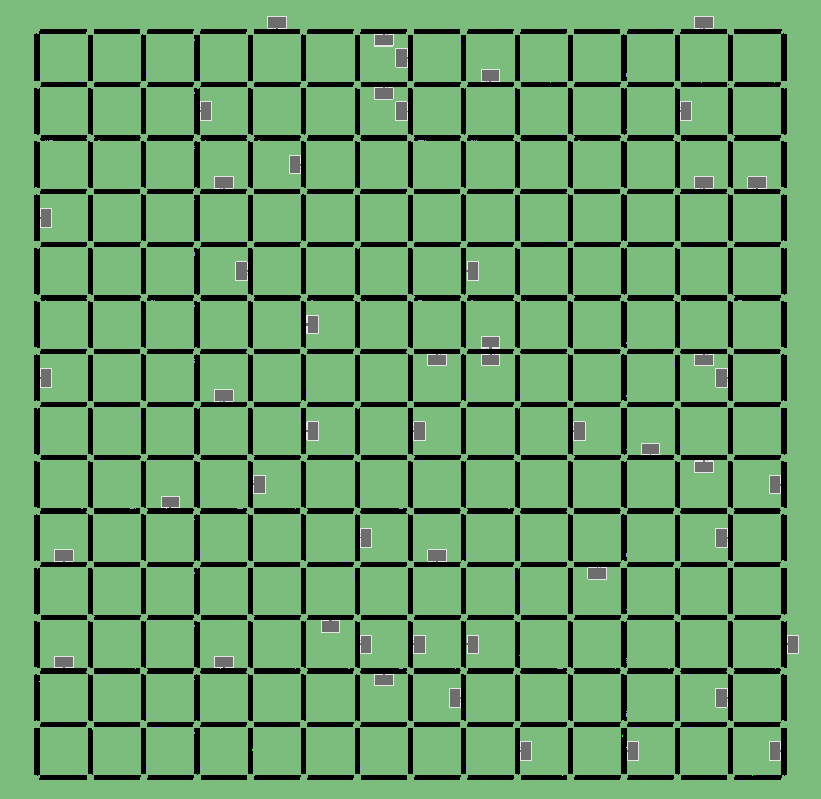
\includegraphics[width=\linewidth]{paper_assets/network_overview.png}
    \caption{包含生成停车设施的 SUMO 整体路网。}
    \label{fig:network_overview}
\end{figure}

\begin{figure}[!t]
    \centering
    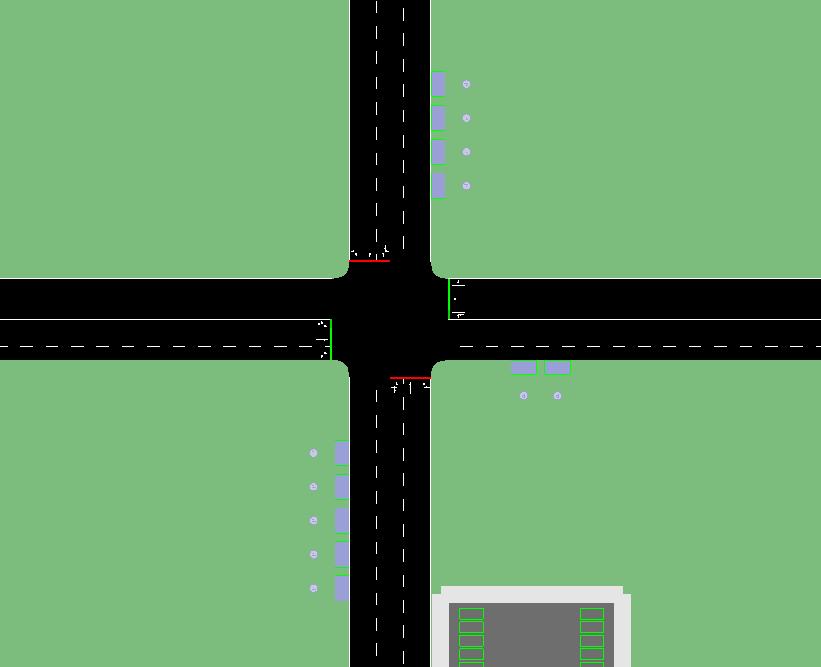
\includegraphics[width=\linewidth]{paper_assets/intersection_detail.png}
    \caption{生成网格路网中的十字路口局部细节。}
    \label{fig:intersection_detail}
\end{figure}

\begin{figure}[!t]
    \centering
    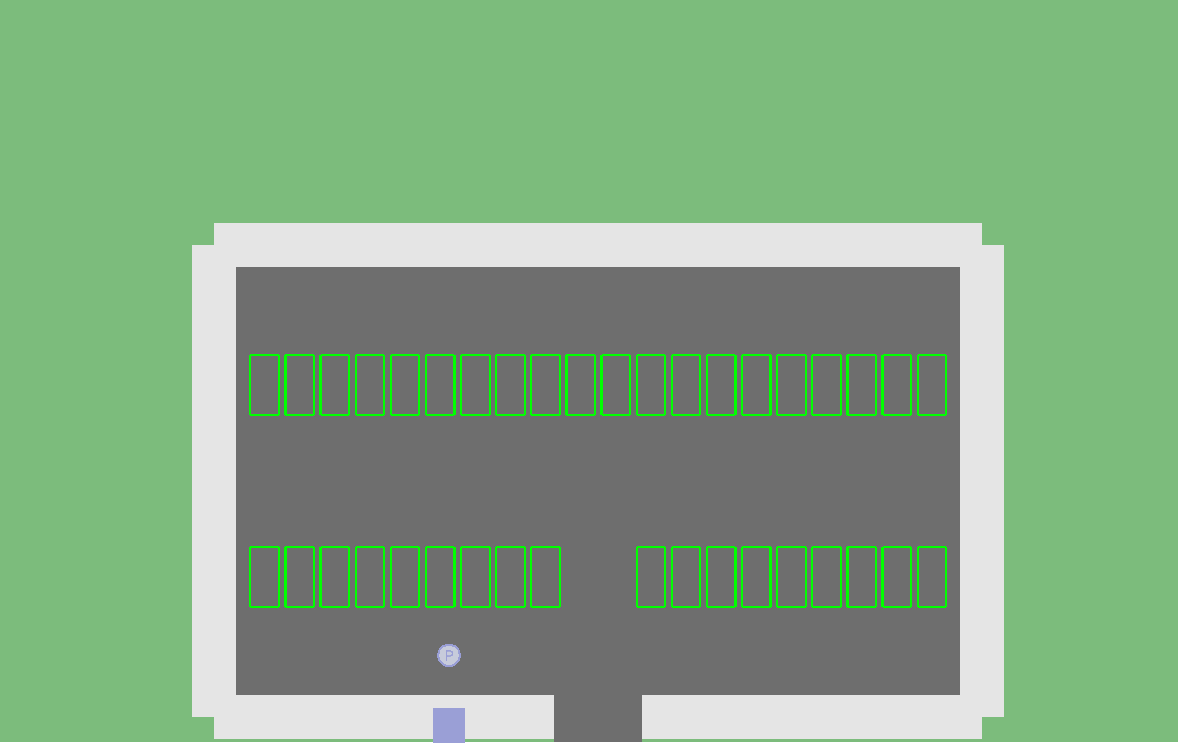
\includegraphics[width=\linewidth]{paper_assets/offstreet_parking_detail.png}
    \caption{停车库存中表示的路外停车场设施。}
    \label{fig:offstreet_detail}
\end{figure}

\subsection{仿真参数}
\begin{table}[htbp]
    \caption{仿真配置参数}
    \label{tab:parameters}
    \centering
    \footnotesize
    \begin{tabular}{|p{0.36\linewidth}|p{0.50\linewidth}|}
        \hline
        \textbf{参数} & \textbf{配置值} \\
        \hline
        仿真器 & Eclipse SUMO \\
        跟驰模型 & Krauss \cite{b10} \\
        车辆总数 & 2,500 \\
        仿真时长 & 7,200 秒（2 小时） \\
        行程出发时间 & \texttt{demo.trips.xml} 中为 3.0--3,599.8 秒 \\
        停车记录数 & 850（800 个路侧，50 个路外枢纽） \\
        物理停车容量 & 2,700 个泊位 \\
        数据库后端 & PostgreSQL 18.4 \\
        控制接口 & 基于 Python 3.10 的 TraCI \\
        定价阈值（$\rho$） & 第 1 层：70\%（1.5 倍），第 2 层：90\%（2.0 倍） \\
        \hline
    \end{tabular}
\end{table}

\begin{table}[htbp]
    \caption{两个场景脚本使用的项目常量}
    \label{tab:implementation_constants}
    \centering
    \footnotesize
    \begin{tabular}{|p{0.42\linewidth}|p{0.42\linewidth}|}
        \hline
        \textbf{实现设置} & \textbf{项目代码中的取值} \\
        \hline
        基线可视寻位距离 & 180 m \\
        基线车位扫描间隔 & 3 个仿真步 \\
        目标等待超时 & 120 秒 \\
        数据库同步间隔 & 60 秒 \\
        智能分配距离成本 & 每米 $0.0025$ 个货币单位 \\
        路侧聚合阈值 & 容量 $\leq 3$ 个泊位 \\
        监控刷新间隔 & 5 个仿真步 \\
        \hline
    \end{tabular}
\end{table}

\subsection{评估场景}
\begin{itemize}
    \item \textbf{场景 A（基线随机搜索）}: 停用智能分配系统。车辆从道路上扫描附近路侧车位，创建待停目标，放弃已不可用车位，并在路径即将耗尽时随机重路由。
    \item \textbf{场景 B（智能分配）}: 启用预约架构。车辆出发时查询状态字典，获得统一货币成本最小的车位，增加预约计数，并以批处理方式把占用和价格同步到 PostgreSQL。
\end{itemize}

\section{结果与性能评估}

图 \ref{fig:scenario_a_monitor} 展示了基线监控面板。六图布局包含实时寻位车辆数、累计成功停车数、显式巡航距离、平均寻车耗时、累计燃油消耗和路网平均速度。该曲线到达两小时边界，而不是完成全部车辆停放：数据库日志记录 2,500 条计划行程中有 2,498 辆成功停车，停车率为 99.92\%，显式巡航距离为 2,692.06 km，平均搜索时间为 371.29 秒。

\begin{figure}[!t]
    \centering
    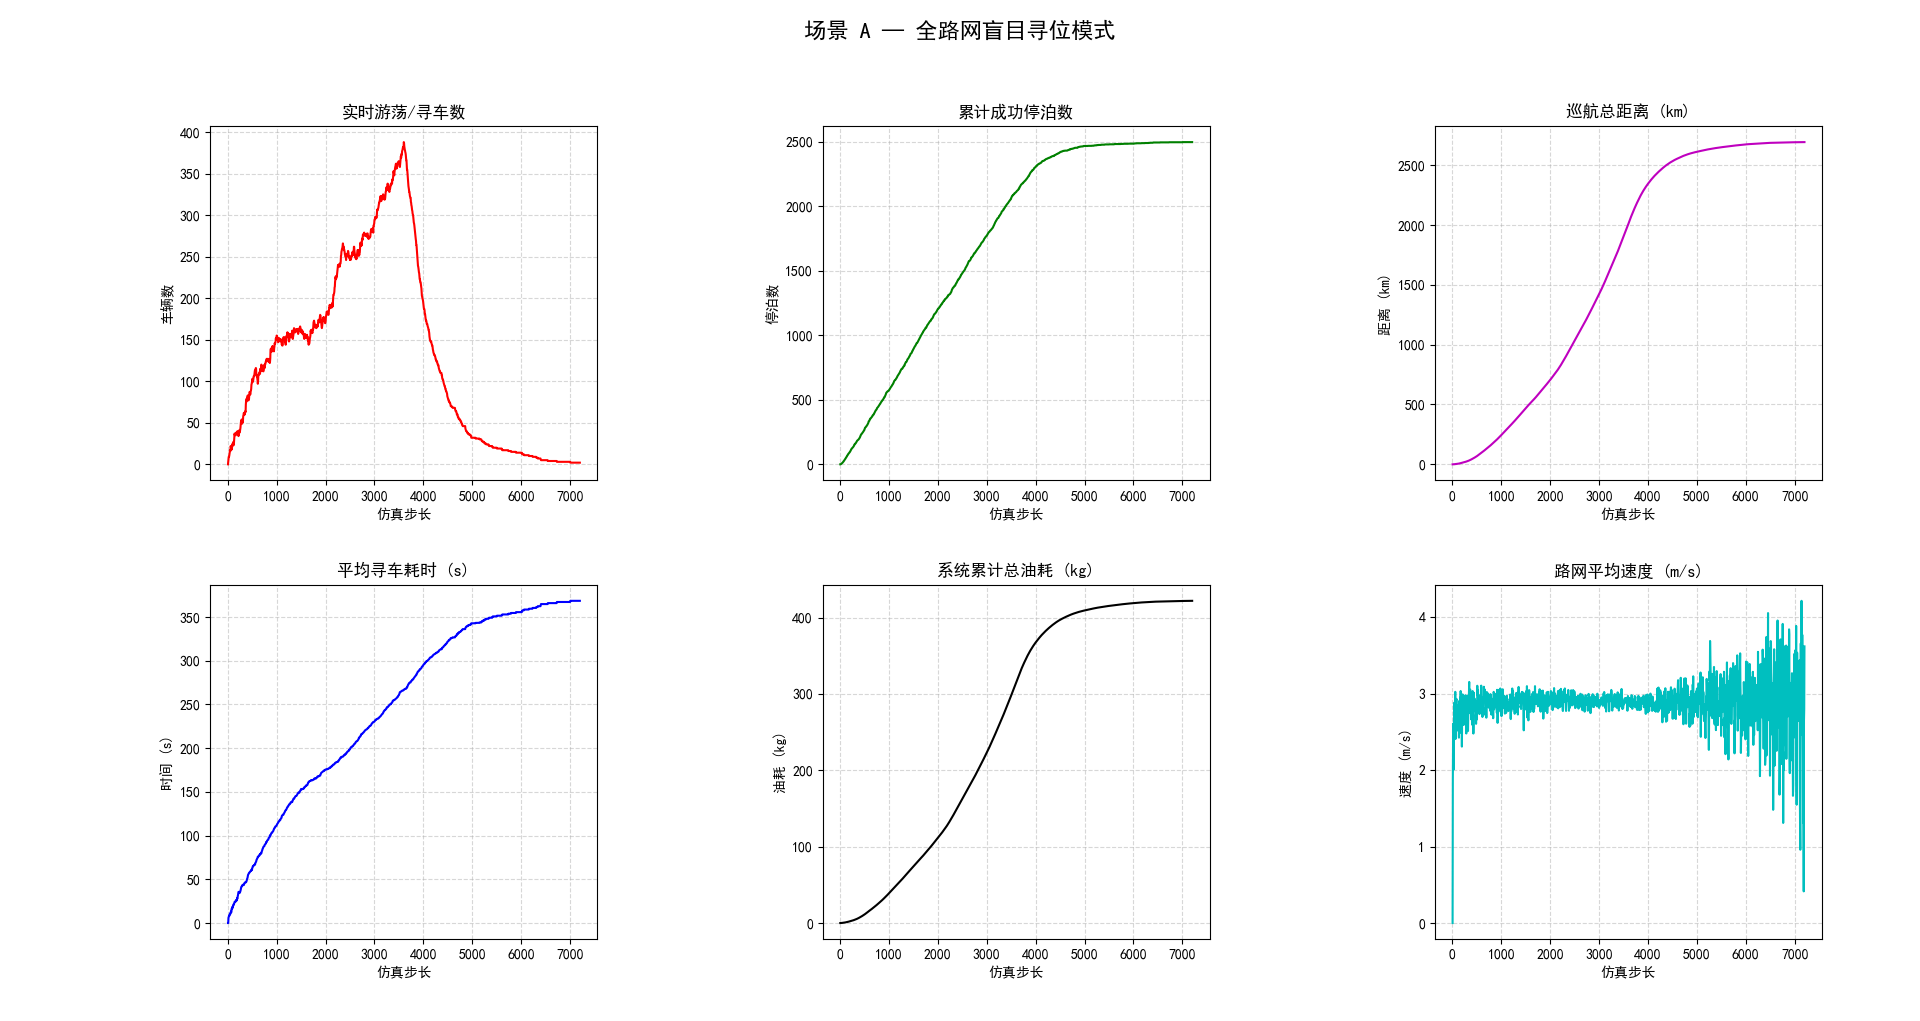
\includegraphics[width=\linewidth]{paper_assets/scenario_A_monitor.png}
    \caption{项目 Matplotlib 监控器生成的场景 A 面板：全路网盲目寻位下的活跃寻位车辆、累计停车、巡航距离、平均寻车耗时、累计燃油与路网速度。}
    \label{fig:scenario_a_monitor}
\end{figure}

图 \ref{fig:scenario_b_monitor} 展示了智能预约监控面板。四图布局关注累计成功停车数、平均寻车耗时、累计燃油消耗和路网平均速度。场景 B 在 3,922 秒完成全部 2,500 辆车停放，停车率为 100.00\%，数据库平均搜索时间为 108.72 秒。

\begin{figure}[!t]
    \centering
    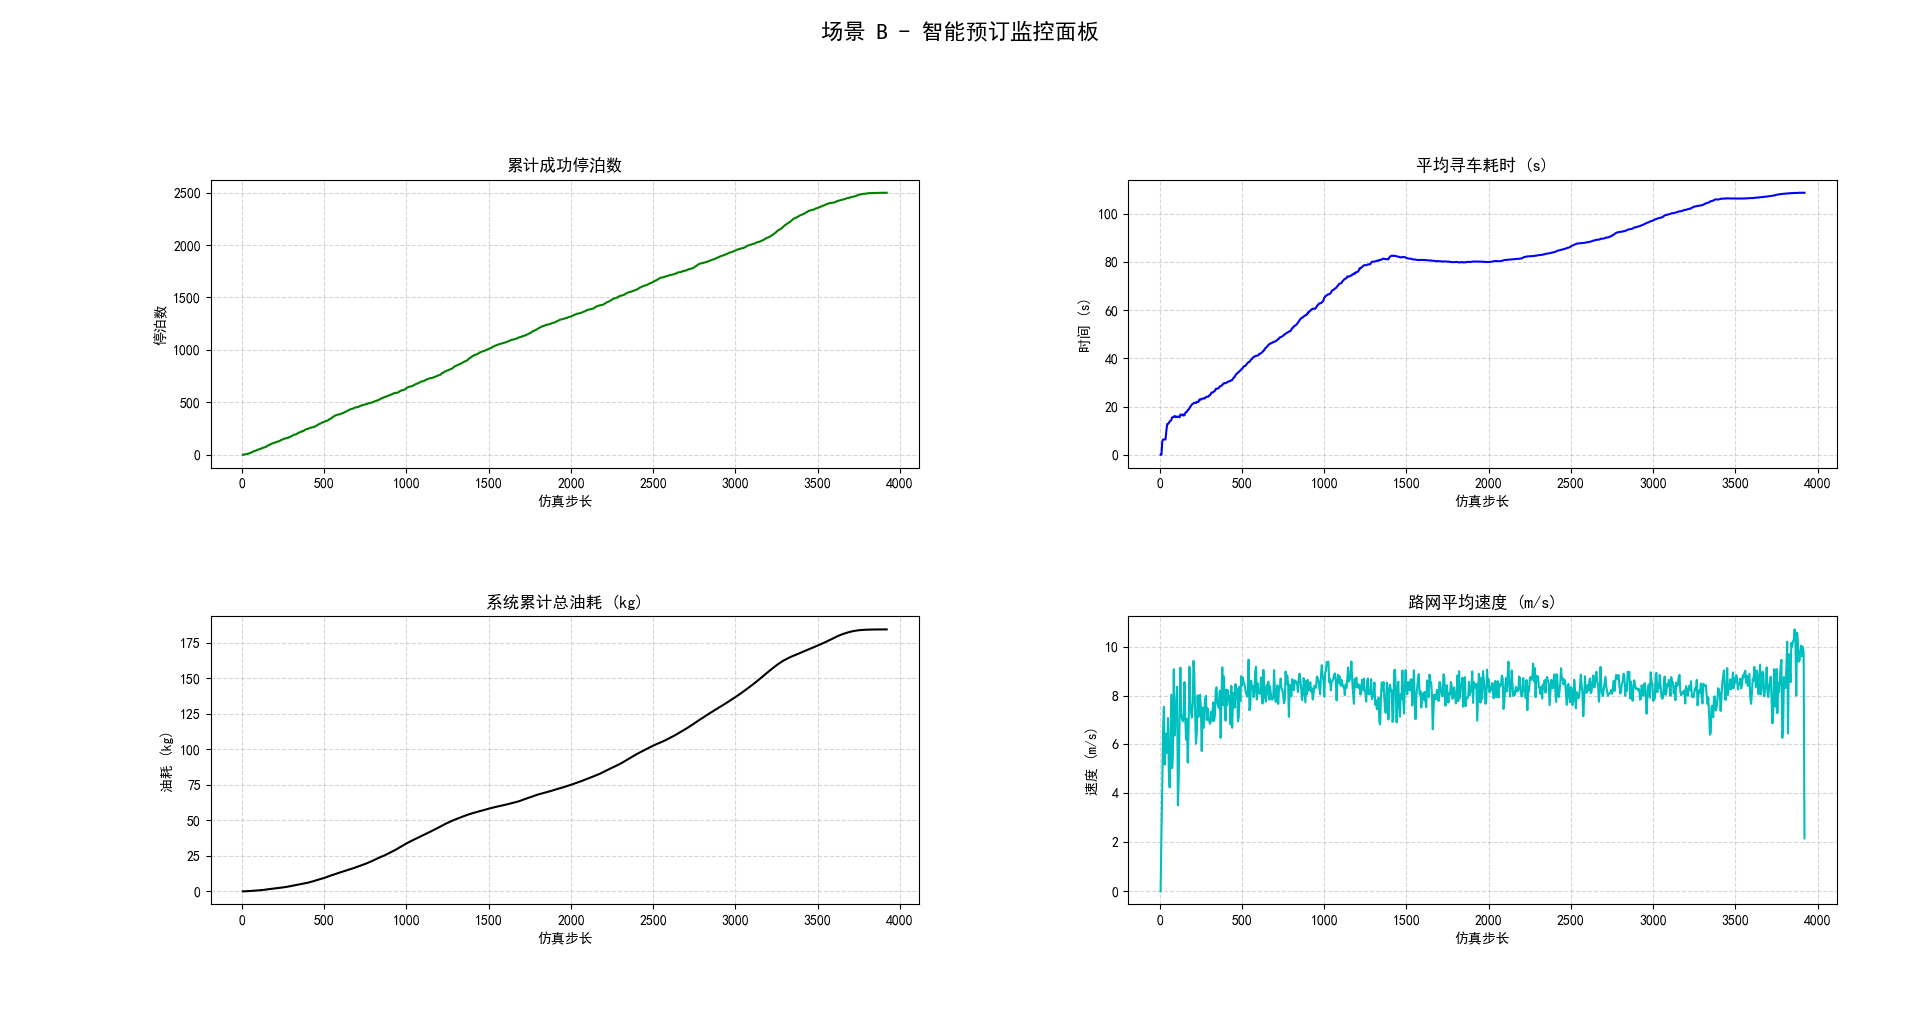
\includegraphics[width=\linewidth]{paper_assets/scenario_B_monitor.png}
    \caption{项目 Matplotlib 监控器生成的场景 B 面板：智能预约下的累计停车、平均寻车耗时、累计燃油与路网速度。}
    \label{fig:scenario_b_monitor}
\end{figure}

评估使用两类数据库来源：\texttt{simulation\_runs} 保存仿真结束时间，\texttt{Cruising\_Logs} 聚合车辆级停车结果、行驶代价、燃油以及 CO$_2$、NOx、PMx 等排放指标。停车率根据车辆级停车记录计算，因此场景 A 被报告为 2,500 条计划行程中有 2,498 辆成功停车。关键运行结果仍然是仿真总时间：场景 B 在 3,922 秒完成全部车辆停放，而场景 A 到达两小时即 7,200 秒仿真上限时，车辆日志中仍有 2 辆未完成停车。

\begin{table}[htbp]
    \caption{停车率与仿真结束时间}
    \label{tab:run_metrics}
    \centering
    \footnotesize
    \begin{tabular}{|p{0.34\linewidth}|c|c|}
        \hline
        \textbf{指标} & \textbf{场景 A} & \textbf{场景 B} \\
        \hline
        计划车辆数 & 2,500 & 2,500 \\
        成功停车车辆 & 2,498 & \textbf{2,500} \\
        未停车车辆 & 2 & \textbf{0} \\
        停车率 & 99.92\% & \textbf{100.00\%} \\
        结束时间（s） & 7,200 & \textbf{3,922} \\
        结束时间（min） & 120.00 & \textbf{65.37} \\
        结束状态 & 达到时限 & 全部停放 \\
        \hline
    \end{tabular}
\end{table}

\begin{table}[htbp]
    \caption{运行与部分环境指标聚合结果}
    \label{tab:vehicle_metrics}
    \centering
    \footnotesize
    \begin{tabular}{|p{0.34\linewidth}|c|c|}
        \hline
        \textbf{指标} & \textbf{场景 A} & \textbf{场景 B} \\
        \hline
        平均搜索时间（s） & 371.29 & \textbf{108.72} \\
        显式巡航距离（km） & 2,692.06 & \textbf{0.00} \\
        总燃油（kg） & 421.87 & \textbf{184.58} \\
        总 CO$_2$（kg） & 1,301.31 & \textbf{569.37} \\
        总 NOx（g） & 413.17 & \textbf{190.02} \\
        总 PMx（g） & 46.53 & \textbf{46.08} \\
        \hline
    \end{tabular}
\end{table}

与基线相比，智能分配将仿真结束时间缩短 3,278 秒，降幅为 45.53\%，并将停车率从 99.92\% 提高到 100.00\%。车辆级日志显示，平均搜索时间降低 70.72\%，预约阶段显式巡航被消除，总燃油与 CO$_2$ 均下降 56.25\%，NOx 下降 54.01\%，PMx 下降 0.97\%。

\section{结论}
本文提出了一种智能停车分配系统，旨在减少“为寻找停车位而巡游”的现象。Python TraCI 控制循环将 SUMO 车辆路由与 PostgreSQL 场景日志、实时预约状态更新和两个可执行 SUMO 场景的仪表盘级对比连接起来。数据库结果显示，场景 A 在 7,200 秒仿真上限时停放 2,498/2,500 辆计划车辆，而场景 B 在 3,922 秒完成全部 2,500 辆车停放。场景 B 因而同时改善停车完成情况和仿真总时间，并使平均搜索时间降低 70.72\%，燃油与 CO$_2$ 降低 56.25\%，NOx 降低 54.01\%，PMx 降低 0.97\%。

\begin{thebibliography}{00}
    \bibitem{b1} D. C. Shoup, ``Cruising for parking,'' \textit{Transport Policy}, vol. 13, no. 6, pp. 479--486, 2006.
    \bibitem{b2} E. Inci, ``A review of the economics of parking,'' \textit{Economics of Transportation}, vol. 4, no. 1-2, pp. 50--63, 2015.
    \bibitem{b3} T. Lin, H. Rivano, and F. Le Mouel, ``A Survey of Smart Parking Solutions,'' \textit{IEEE Transactions on Intelligent Transportation Systems}, vol. 18, no. 12, pp. 3229--3253, Dec. 2017.
    \bibitem{b4} Y. Geng and C. G. Cassandras, ``New smart parking system based on resource allocation and reservations,'' \textit{IEEE Transactions on Intelligent Transportation Systems}, vol. 14, no. 3, pp. 1129--1139, 2013.
    \bibitem{b5} R. Arnott and J. Rowse, ``Modeling parking,'' \textit{Journal of Urban Economics}, vol. 45, no. 1, pp. 97--124, 1999.
    \bibitem{b6} M. Fosgerau and A. de Palma, ``The dynamics of urban traffic congestion and the price of parking,'' \textit{Journal of Public Economics}, vol. 105, pp. 106--115, 2013.
    \bibitem{b7} G. Pierce and D. Shoup, ``Getting the prices right: An evaluation of pricing parking by demand in San Francisco,'' \textit{Journal of the American Planning Association}, vol. 79, no. 1, pp. 67--81, 2013.
    \bibitem{b8} A. Wegener, M. Piórkowski, M. Raya, H. Hellbrück, S. Fischer, and J.-P. Hubaux, ``TraCI: an interface for coupling road traffic and network simulators,'' \textit{Proceedings of the 11th Communications and Networking Simulation Symposium}, 2008, pp. 155--163.
    \bibitem{b10} S. Krauss, ``Microscopic modeling of traffic flow: Investigation of collision free vehicle dynamics,'' Ph.D. dissertation, DLR, Cologne, Germany, 1998.
    \bibitem{b11} M. Behrisch, L. Bieker, J. Erdmann, and D. Krajzewicz, ``SUMO Simulation of Urban Mobility: An Overview,'' \textit{Proceedings of SIMUL 2011, The Third International Conference on Advances in System Simulation}, 2011.
\end{thebibliography}

\end{document}




